\documentclass[8pt]{beamer}
\usetheme{Madrid}
\usefonttheme{serif}

\usepackage{fontspec}
% надёжный шрифт с кириллицей (работает в Overleaf)
\setmainfont{Libertinus Serif}[Ligatures=TeX]
\setsansfont{Libertinus Sans}[Ligatures=TeX]
\newfontfamily\cyrillicfont{Libertinus Serif}
\newfontfamily\cyrillicfontsf{Libertinus Sans}
\usepackage{polyglossia}
\setmainlanguage{russian}
\setotherlanguage{english}

\usepackage{amsmath}
\usepackage{amsfonts}
\usepackage{amssymb}
\usepackage{graphicx}
\usepackage{microtype}

\usepackage{tabularx}
\usepackage{booktabs}

\usepackage{xcolor}
\usepackage{pifont}
\usepackage{tikz}
\newcommand{\plus}{\tikz[baseline=(X.base)] \node[fill=green!65!black, rounded corners=2pt, inner sep=2pt] (X) {\color{white}\ding{51}};}
\newcommand{\minus}{\tikz[baseline=(X.base)] \node[fill=red!70!black,   rounded corners=2pt, inner sep=2pt] (X) {\color{white}\ding{55}};}

\DeclareMathOperator{\sen}{sen}
% \DeclareMathOperator{\tg}{tg}

\setbeamertemplate{caption}[numbered]

% --- Информация о презентации ---
\author[Автор]{Чиняев Владимир Николаевич}
\title{Моделирование множественных протяженных маневров \\ с учетом возмущающих сил}
\newcommand{\coursename}{Введение в маневрирование КА}
\setbeamertemplate{navigation symbols}{} 
\institute[]{Московский физико технический институт} 
\date{18 ноября 2025 г.} 

\bibliographystyle{apalike}

% --- Кастомная нижняя синяя полоска: курс слева, номер слайда справа ---
\setbeamertemplate{footline}{
  \leavevmode%
  \begin{beamercolorbox}[wd=\paperwidth,ht=2ex,dp=1ex]{palette primary}
    \hspace{0.4cm}\usebeamerfont{footline}\coursename\hfill\usebeamerfont{footline}\insertframenumber\hspace{0.4cm}
  \end{beamercolorbox}%
}

% Чтобы убрать лишние отступы в footer-шрифте (опционально)
\setbeamerfont{footline}{size=\small}

\begin{document}

\begin{frame}
\titlepage
\end{frame}

\begin{frame}{Почему изученные методы решения задач недостаточны?}
На предыдущих лекциях мы решали задачи маневрирования в следующих предположениях:
\begin{itemize}
    \item Манёвры импульсные;
    \item КА движется в точечном потенциале.
\end{itemize}
В реальности:
\begin{itemize}
    \item ДУ КА имеет конечную тягу, а потому требуемый импульс $\Delta V$ прикладывается за некоторое конечное время (иногда очень продолжительное);
    \item Движение КА определяется целым набором сил: Земная гравитация, притяжение третьих тел (Солнце, Луна), сопротивление атмосферы и тд.  
\end{itemize}
\end{frame}

\begin{frame}{Преобразование импульсного манёвра в протяжённый}
Если манёвр выполняется в фиксированном направлении в инерциальной СК, а $\Delta V$ распределён по дуге орбиты с центральным углом $\theta$, то эффективность такого манёвра можно оценить так:
\begin{equation*}
    \kappa = \frac{\sin \theta / 2}{\theta / 2}.
\end{equation*}
\begin{itemize}
    \item При малой дуге (малое $\theta$) $\kappa \rightarrow 1$: конечный манёвр близок к импульсному;
    \item При большой длительности (большом $\theta$) эффективность падает: та же величина $\Delta V$ даёт меньший эффект на элементы орбиты.
\end{itemize}
Эта формула является приближённой и получена в следующих предположениях: околокруговые орбиты, манёвры малы, отклонения от плоскости малы и тд.
\begin{table}[h]
    \centering
    \scriptsize
    \begin{tabular}{|c|cccccccccccc|}
        \hline
        $\theta,^\circ$
            & 5 & 10 & 15 & 20 & 40 & 60 & 80 & 100 & 120 & 140 & 160 & 180 \\ \hline
        $\kappa$
            & 0.9997 & 0.9987 & 0.9971 & 0.9949
            & 0.9798 & 0.9549 & 0.9207 & 0.8778
            & 0.8270 & 0.7691 & 0.7053 & 0.6366 \\ \hline
        $1 - \kappa$, \%
            & 0.03 & 0.13 & 0.29 & 0.51
            & 2.02 & 4.51 & 7.93 & 12.22
            & 17.30 & 23.09 & 29.47 & 36.34 \\ \hline
    \end{tabular}
\end{table}
Способы уменьшить потери эффективности при переходе к протяжённым манёврам:
\begin{itemize}
    \item Увеличить тягу ДУ (сократить длительность и дугу);
    \item Использовать оптимальную ориентацию вектора тяги в каждой точке орбиты;
    \item Разбить один большой манёвр на несколько маленьких, тем самым уменьшив дугу каждого.
\end{itemize}
\end{frame}

\begin{frame}{Ошибки выполнения манёвров}
Когда манёвр планируется, вычисляется \textbf{номинальное} постманевровое состояние, которое будет достигнуто при полностью оптимальном выполнении манёвра. После того, как манёвр был совершён, необходимые данные собраны и обработаны, вычисляется \textbf{наблюдаемое} постманевровое состояние. Разница между наблюдаемым и номинальным состояниями называется \textbf{ошибкой выполнения манёвра}. 
\begin{center}
\boxed{
    \textbf{Манёвры никогда не выполняются идеально!} 
}
\end{center}
Источники ошибок:
\begin{itemize}
    \item Неточности определения орбиты КА;
    \item Неточности определения или управления ориентацией КА;
    \item Неточности в работе ДУ (значение тяги, температура газов, время работы и тд.);
    \item Неточности во времени выполнения манёвра.
\end{itemize}
Хорошо, если ошибки выполнения манёвров малы, но они могут быть и достаточно велики. 

\bigskip

\textbf{Простой пример}. Пусть ДУ имеет ошибку в $1\%$ по величине импульса. Тогда ошибка $1\%$ от манёвра с величиной $1 \; \text{м/с}$ составит лишь $0.01 \; \text{м/с}$. С другой стороны, ошибка $1\%$ от манёвра с величиной $800 \; \text{м/с}$ это $8 \; \text{м/с}$.
\end{frame}

\begin{frame}{Группа манёвров и её структура}
\textbf{Группа манёвров} - набор манёвров, выполняемых на последовательных витках примерно в одной и той же точке орбиты и в одной и той же ориентации, с целью выполнения одного «большого» манёвра.

Зачем разбивать манёвр на несколько манёвров?
\begin{itemize}
    \item Уменьшить потери в эффективности при переходе от импульсных к протяжённым манёврам;
    \item Снизить чувствительность к ошибкам исполнения манёвров.
\end{itemize}

Существуют два сценария после выполнения манёвра:
\begin{itemize}
    \item \textbf{Впереди есть запланированные манёвры}. \\
    Параметры последующих манёвров можно пересчитать, для того, чтобы скомпенсировать ошибку выполнения текущего манёвра;
    \item \textbf{Выполненный манёвр был последним}. \\
    Ошибка выполнения такого манёвра напрямую сказывается на ошибке достижения КА целевого состояния/орбиты.
\end{itemize}
\end{frame}

\begin{frame}{Группа манёвров и её структура}
Возникает новый вопрос: как преобразовать одиночный манёвр в группу манёвров?
\begin{columns}[T,totalwidth=\textwidth]
  % Левая колонка
  \begin{column}{0.50\textwidth}
    \begin{center}
        \textbf{Поделить манёвр на одинаковые части}
    \end{center}
    \plus\ Самый эффективный вариант с точки зрения перехода от импульсных манёвров к протяжённым; \\
    \minus\ Ошибки выполнения манёвров могут быть существенными, особенно при выполнении последнего манёвра в группе.
  \end{column}

  % Правая колонка
  \begin{column}{0.50\textwidth}
    \begin{center}
        \textbf{Последовательно уменьшать величину манёвров}
    \end{center}
    \minus\ Менее эффективен с точки зрения перехода от импульсных манёвров к протяжённым; \\
    \plus\ Даёт возможность корректировать ошибки выполнения первых "больших манёвров" последующими, меньшими по величине манёврами. Позволяет гибко корректировать ошибку последнего манёвра.
  \end{column}
\end{columns}
Рекомендуется использовать такую структуру группы: плавно уменьшать величину $\Delta V$ от первого к последнему манёвру. Можно использовать следующее правило:
\begin{equation*}
    w_{i+1} = k w_i,
\end{equation*}
где $w_i$ - вес $i$-го манёвра группы, $0 < k < 1$. Тогда величина каждого манёвра может быть посчитана так:
\begin{equation*}
    \Delta V_i = \Delta V_\Sigma \frac{w_i}{\sum_j w_j}.
\end{equation*}
Величина $k$ подбирается так, чтобы:
\begin{itemize}
    \item Каждый последующий манёвр мог компенсировать ошибку выполнения предыдущего манёвра;
    \item Последний манёвр в группе был достаточно точным (ошибка его выполнения была достаточно мала), чтобы обеспечить достижение целевого состояния/орбиты.
\end{itemize}
\end{frame}

\begin{frame}{Переработка/недоработка ДУ}
\begin{center}
    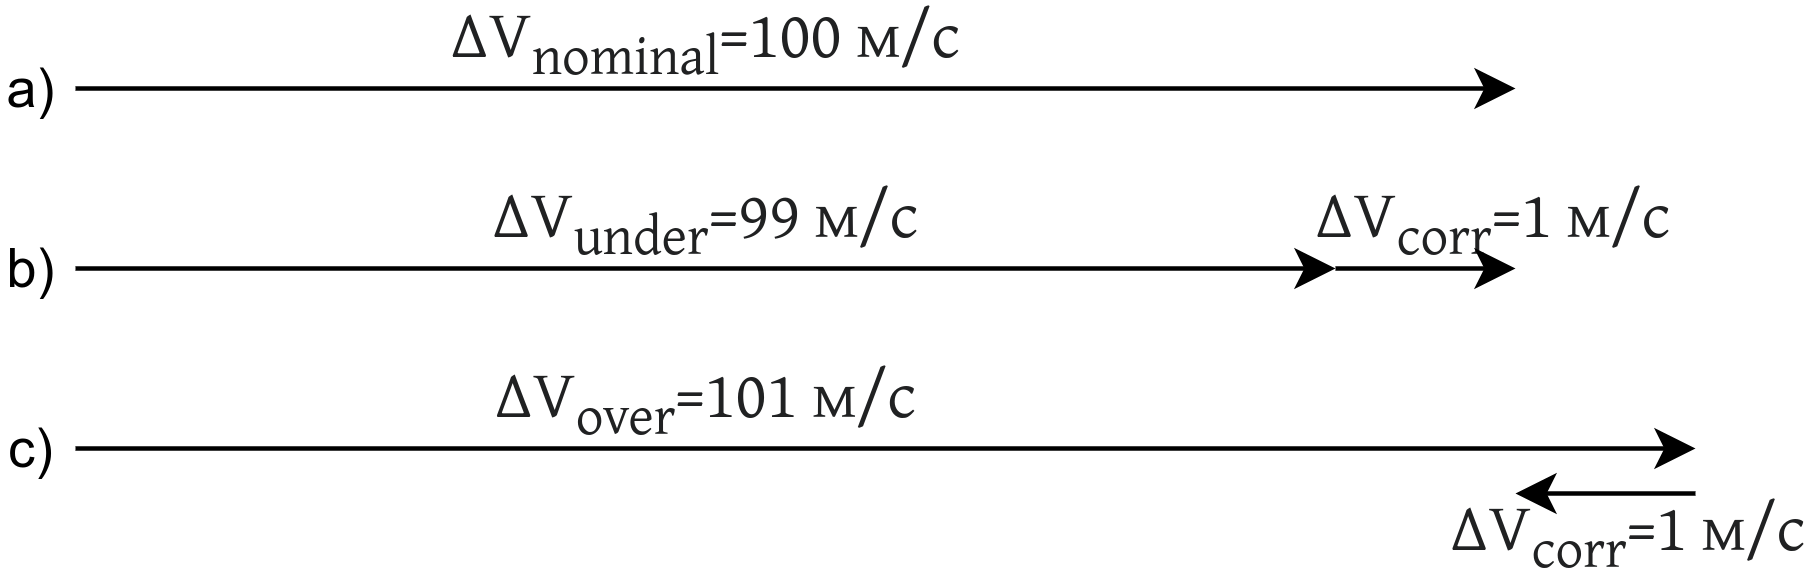
\includegraphics[height=0.25\textheight,keepaspectratio]{images/9/perf_image.png}
\end{center}
Что предпочтительнее, переработка или недоработка ДУ? Рассмотрим рисунок выше. 
\begin{itemize}
    \item Недоработка в $1\%$. \\
    Требуется корректирующий импульс $\Delta V_{\text{corr}} = 1 \text{м/с}$ в \textbf{том же направлении}. Тогда суммарная величина импульса $\Delta V_{\text{under}} + \Delta V_{\text{corr}} = \Delta V_{\text{nominal}}$.
    \item Переработка в $1\%$. \\
    Требуется корректирующий импульс $\Delta V_{\text{corr}} = 1 \text{м/с}$ в \textbf{противоположном направлении}. Тогда суммарная величина импульса $\Delta V_{\text{over}} + \Delta V_{\text{corr}} > \Delta V_{\text{nominal}}$.
\end{itemize}
Существуют и такие примеры, где переработка ДУ позволит получить выгоду. Поэтому предпочтительность будет зависеть от конкретной задачи.
\end{frame}

\begin{frame}{Исполнение группы протяжённых манёвров}
Для того, чтобы выполнить маневрирование необходимы:
\begin{itemize}
    \item Начальные условия: состояние КА, начальная эпоха;
    \item Набор протяжённых манёвров: времена начала и окончания манёвров, профиль тяги ДУ, ориентация КА;
    \item Параметры КА: масса, тяга ДУ, максимальная/минимальная продолжительность импульса, минимальное время между импульсами, ограничения на количество импульсов, ограничения на ориентацию КА;
\end{itemize}
Сценарий выполнения маневрирования:
\begin{itemize}
    \item Прогноз пассивного движения КА с учётом различных возмущающих сил;
    \item Прогноз активного движения КА: пассивные силы + сила тяги ДУ.
\end{itemize}
\end{frame}

\begin{frame}{Высокоточный прогноз движения КА}
Для того, чтобы полученное решение было применимо в реальности, необходимо использовать баллистический прогноз движения КА, учитывающий широкий спектр сил: 
\begin{itemize}
    \item Гравитационное поле Земли ($16 \times 16$, $32 \times 32$, $64 \times 64$ гармоник разложения геопотенциала);
    \item Притяжение Луны и Солнца;
    \item Сопротивление атмосферы;
    \item Влияние излучения и тд.
\end{itemize}
Важно отметить, что на различных этапах решения задачи маневрирования, удобно пользоваться "подходящими" моделями сил, используемыми для баллистического прогноза. Например, оптимизацию решения удобнее производить в "упрощённой" модели сил: точечный потенциал + импульсные манёвры или $\text{J}_2$ + импульсные манёвры. Единственное требование: \textbf{упрощённое решение должно учитывать основные особенности решаемой задачи}. 
\end{frame}

\begin{frame}[allowframebreaks]{Источники}
  \begin{thebibliography}{9}

    \bibitem{DiPrinzio}
    DiPrinzio M. Methods of Orbital Maneuvering. – American Institute of Aeronautics and Astronautics, Inc., 2019.
    
  \end{thebibliography}
\end{frame}

\end{document}